\documentclass[12pt,letterpaper]{exam}
\usepackage[lmargin=1in,rmargin=1in,tmargin=1in,bmargin=1in]{geometry}
\usepackage{../style/exams}

% -------------------
% Course & Exam Information
% -------------------
\newcommand{\course}{MAT 101: Exam 2}
\newcommand{\term}{Summer -- 2022}
\newcommand{\examdate}{06/02/2022}
\newcommand{\timelimit}{85 Minutes}

\setbool{hideans}{false} % Student: True; Instructor: False

% -------------------
% Content
% -------------------
\begin{document}

\examtitle
\instructions{Write your name on the appropriate line on the exam cover sheet. This exam contains \numpages\ pages (including this cover page) and \numquestions\ questions. Check that you have every page of the exam. Answer the questions in the spaces provided on the question sheets. Be sure to answer every part of each question and show all your work.} 
\scores
%\bottomline
\newpage

% ---------
% Questions
% ---------
\begin{questions}

% Question 1
\newpage
\question[10] Determine whether the relations $f(x)$ and $g(x)$ shown below are functions. If the relation is a function, explain why. If the relation is not a function, explain why not. 
	\[
	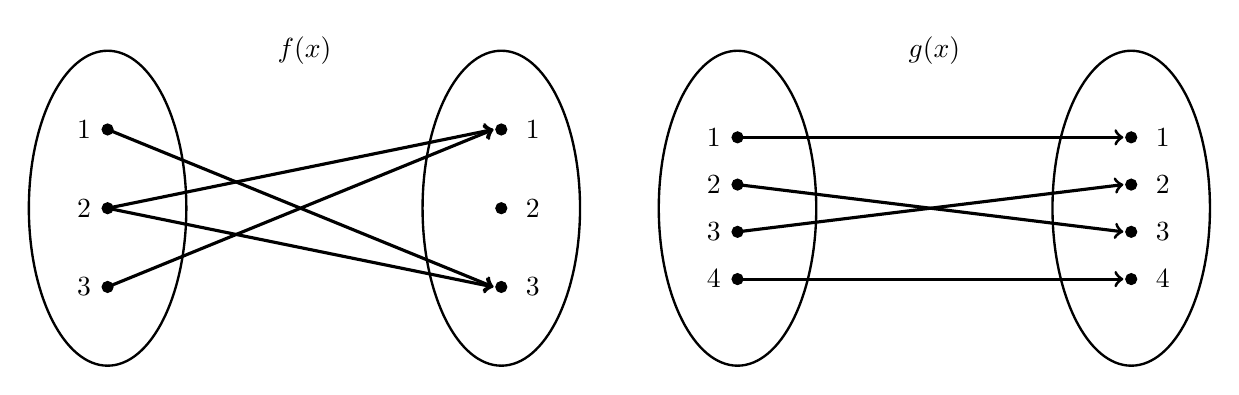
\begin{tikzpicture}
	\node at (2.5,2) {$f(x)$};
	% Ellipses
	\draw[line width=0.03cm] (0,0) circle (1 and 2);
	\draw[line width=0.03cm] (5,0) circle (1 and 2);
	
	% Nodes
	\draw[fill=black] (0,1) circle (0.07);
	\draw[fill=black] (0,0) circle (0.07);
	\draw[fill=black] (0,-1) circle (0.07);
	
	\draw[fill=black] (5,1) circle (0.07);
	\draw[fill=black] (5,0) circle (0.07);
	\draw[fill=black] (5,-1) circle (0.07);
	
	% Arrow
	\draw[line width=0.04cm,->] (0,1) -- (4.9,-1);
	\draw[line width=0.04cm,->] (0,0) -- (4.9,1);
	\draw[line width=0.04cm,->] (0,0) -- (4.9,-1);
	\draw[line width=0.04cm,->] (0,-1) -- (4.9,1);
	
	% Labels
	\node at (-0.3,1) {$1$};
	\node at (-0.3,0) {$2$};
	\node at (-0.3,-1) {$3$};
	
	\node at (5.4,1) {$1$};
	\node at (5.4,0) {$2$};
	\node at (5.4,-1) {$3$};
	
	\tikzset{shift={(8,0)}}
	%
	\node at (2.5,2) {$g(x)$};
	% Ellipses
	\draw[line width=0.03cm] (0,0) circle (1 and 2);
	\draw[line width=0.03cm] (5,0) circle (1 and 2);
	
	% Nodes
	\draw[fill=black] (0,0.9) circle (0.07);
	\draw[fill=black] (0,0.3) circle (0.07);
	\draw[fill=black] (0,-0.3) circle (0.07);
	\draw[fill=black] (0,-0.9) circle (0.07);
	
	\draw[fill=black] (5,0.9) circle (0.07);
	\draw[fill=black] (5,0.3) circle (0.07);
	\draw[fill=black] (5,-0.3) circle (0.07);
	\draw[fill=black] (5,-0.9) circle (0.07);
	
	% Arrow
	\draw[line width=0.04cm,->] (0,0.9) -- (4.9,0.9);
	\draw[line width=0.04cm,->] (0,0.3) -- (4.9,-0.3);
	\draw[line width=0.04cm,->] (0,-0.3) -- (4.9,0.3);
	\draw[line width=0.04cm,->] (0,-0.9) -- (4.9,-0.9);

	
	% Labels
	\node at (-0.3,0.9) {$1$};
	\node at (-0.3,0.3) {$2$};
	\node at (-0.3,-0.3) {$3$};
	\node at (-0.3,-0.9) {$4$};
	
	\node at (5.4,0.9) {$1$};
	\node at (5.4,0.3) {$2$};
	\node at (5.4,-0.3) {$3$};
	\node at (5.4,-0.9) {$4$};
	\end{tikzpicture}
	\] \pspace

{\noindent \itshape Because the relation $f(x)$ has an input with more than one output, i.e. ill-defined inputs, $f(x)$ is not a function. For example, $f(2)$ is not well-defined because $f(2) \in \{ 1, 3 \}$. However, the relation $g(x)$ has only one possible output for each possible input, $g(x)$ is a function. We have\dots
	\[
	\begin{aligned}
	g(1)&= 1 \\
	g(2)&= 3 \\
	g(3)&= 2 \\
	g(4)&= 4
	\end{aligned}
	\]
}



% Question 2
\newpage
\question[10] Determine whether the relation shown below is a function. If the relation is a function, explain why. If the relation is not a function, explain why not. 
	\[
	\fbox{
	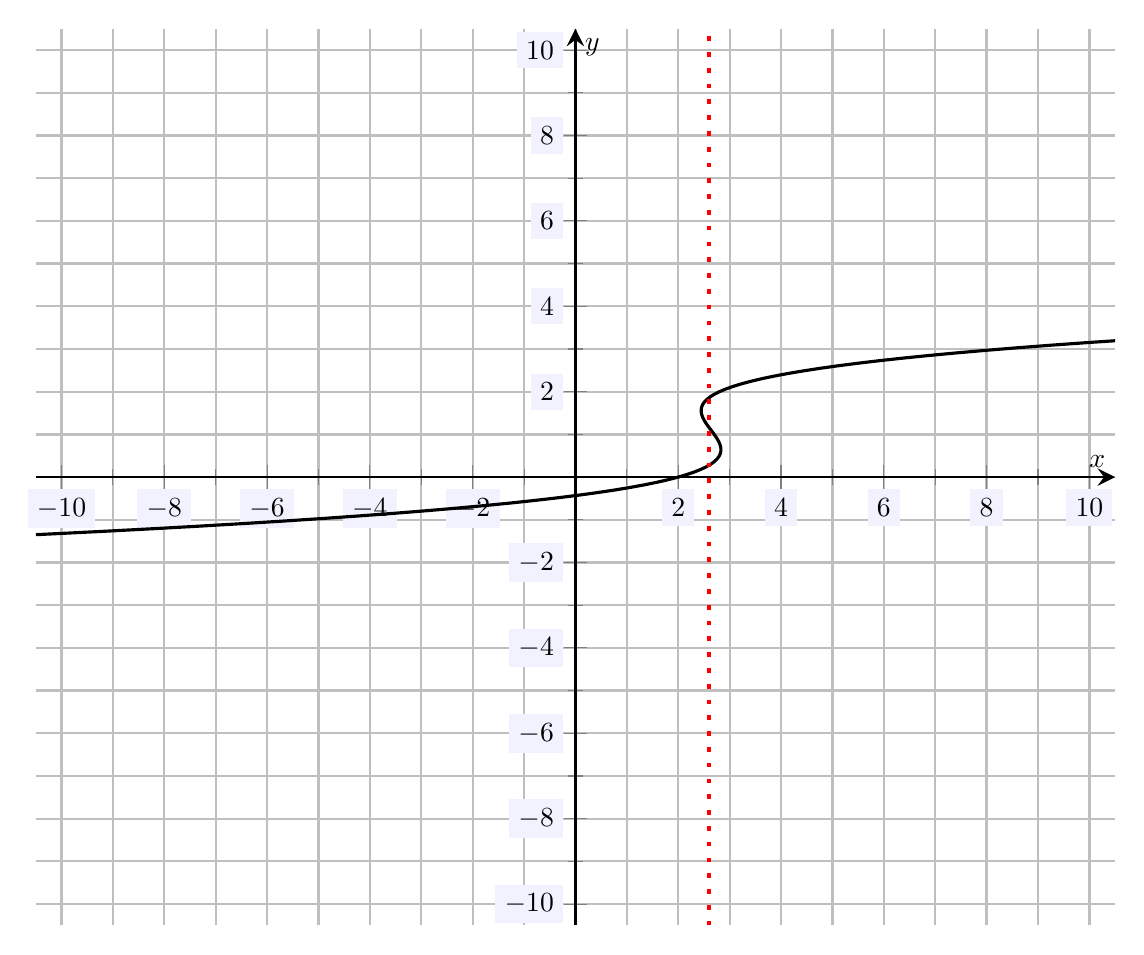
\begin{tikzpicture}[scale=2,every node/.style={scale=0.5}]
	\begin{axis}[
	grid=both,
	axis lines=middle,
	ticklabel style={fill=blue!5!white},
	xmin= -10.5, xmax=10.5,
	ymin= -10.5, ymax=10.5,
	xtick={-10,-8,-6,-4,-2,0,2,4,6,8,10},
	ytick={-10,-8,-6,-4,-2,0,2,4,6,8,10},
	minor tick = {-10,-9,...,10},
	xlabel=\(x\),ylabel=\(y\),
	]
	\addplot[line width= 0.02cm,domain= -2:4, samples=100] ({x^3 - 3.3*x^2 + 3*x + 2},{x}); 
	\draw[red, dotted, line width= 0.03cm] (2.6,-10.5) -- (2.6,10.5);
	\end{axis}
	\end{tikzpicture}
	}
	\] \pspace

{\noindent \itshape Because the relation above does not pass the vertical line test, i.e. every vertical line intersects the curve at most once, the relation is not a function. For instance, the vertical line at $x \approx 2.6$ intersects the curve three times.}



% Question 3
\newpage
\question[10] For the relation shown below, determine the $x$ and $y$-intercepts. 
	\[
	\fbox{
	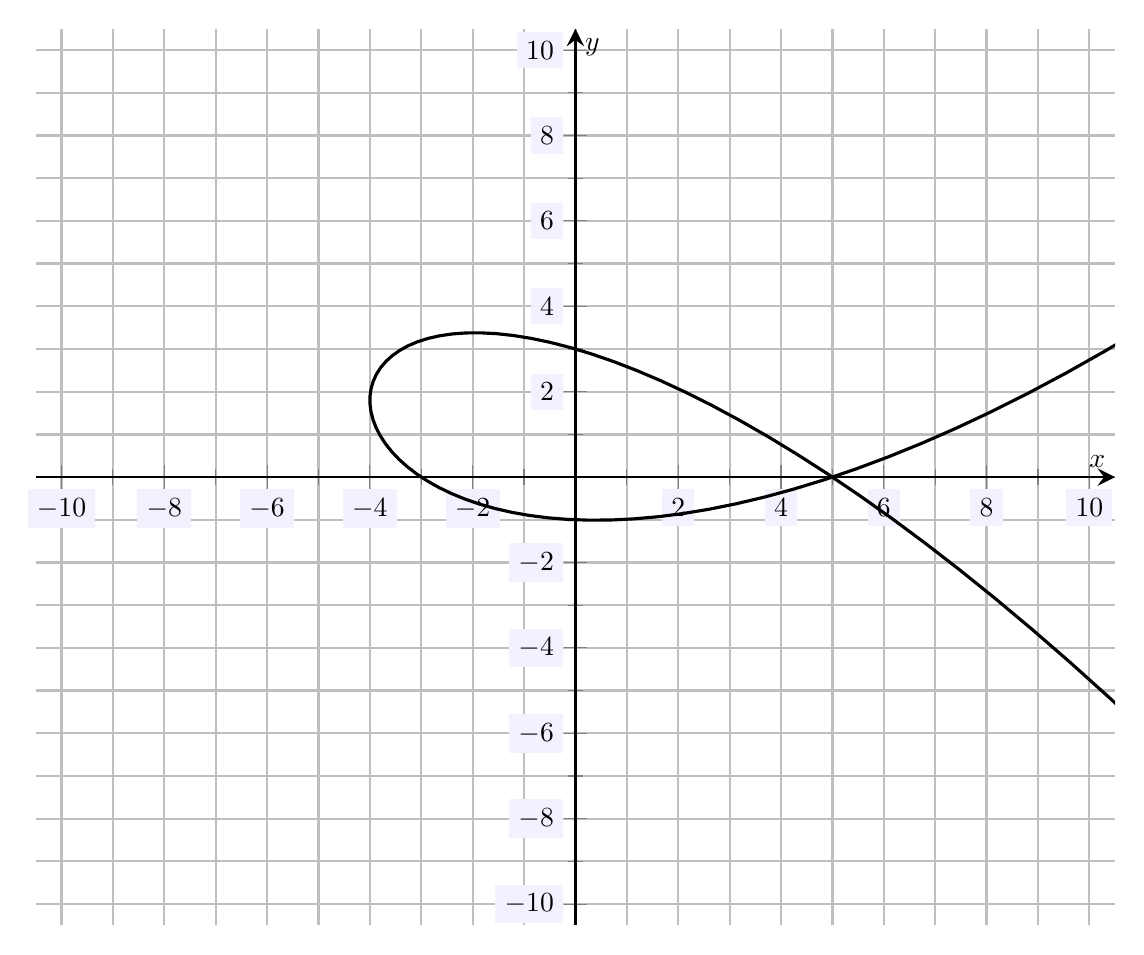
\begin{tikzpicture}[scale=2,every node/.style={scale=0.5}]
	\begin{axis}[
	grid=both,
	axis lines=middle,
	ticklabel style={fill=blue!5!white},
	xmin= -10.5, xmax=10.5,
	ymin= -10.5, ymax=10.5,
	xtick={-10,-8,-6,-4,-2,0,2,4,6,8,10},
	ytick={-10,-8,-6,-4,-2,0,2,4,6,8,10},
	minor tick = {-10,-9,...,10},
	xlabel=\(x\),ylabel=\(y\),
	]
	\addplot[line width= 0.02cm,domain= -10:10, samples=100] ({1/4*(x - 3)*(x + 5)},{1/40*(x - 5)*(x - 1)*(x + 7)}); 
	\end{axis}
	\end{tikzpicture}
	}
	\] \pspace

{\noindent \itshape The $x$-intercepts are the points where the curve intersects the $x$-axis. Therefore, the $x$-intercepts are $(-3, 0)$ and $(5, 0)$. The $y$-intercepts are the points where the curve intersects the $y$-axis. Therefore, the $x$-intercepts are $(0, -1)$ and $(0, 3)$.
	\[
	\boxed{
	\begin{aligned}
	x\text{-intercepts}&\colon (-3, 0),\ (5, 0) \\
	y\text{-intercepts}&\colon (0, -1),\ (0, 3)
	\end{aligned}
	}
	\]
}



% Question 4
\newpage
\question[10] Suppose $f(x)$, $g(x)$, and $h(x)$ are functions whose values are given below.
        \begin{table}[!ht]
        \centering
        \begin{tabular}{| c || r | r | r | r | r | r | r |} \hline
	$x$ & $-5$ & $-3$ & $-1$ & $\phantom{-}0$ & $\phantom{-}2$ & $\phantom{-}6$ & $\phantom{-}10$ \\ \hline \hline
	$f(x)$ & $7$ & $10$ & $0$ & $\tfrac{2}{3}$ & $-4$ & $2$ & $\sqrt{2}$ \\ \hline
	$g(x)$ & $0$ & $\pi$ & $6$ & $\tfrac{4}{5}$ & $1$ & $-3$ & $4$ \\ \hline
	$h(x)$ & $\tfrac{9}{8}$ & $0$ & $-3$ & $-1$ & $-1$ & $8$ & $-8$ \\ \hline
        \end{tabular}
        \end{table}

Compute the following, simplifying as much as possible: \pspace
        \begin{enumerate}[(a)]
        \item $(f + h)(-1)= f(-1) + h(-1)= 0 + -3= -3$ \vfill
        \item $(h - f)(10)= h(10) - f(10)= -8 - \sqrt{2}$ \vfill
        \item $(-2g)(2)= -2g(2)= -2 \cdot 1= -2$ \vfill
        \item $\left( \dfrac{h}{f} \right)(0)= \dfrac{h(0)}{f(0)}= \dfrac{-1}{\tfrac{2}{3}}= -1 \cdot \dfrac{3}{2}= -\dfrac{3}{2}$ \vfill
        \item $g(-3)\, h(6)= \pi \cdot 8= 8\pi$ \vfill
        \item $h(2 - f(2))= h \big(2 - (-4) \big)= h(2 + 4)= h(6)= 8$ \vfill
        \item $(g \circ h)(0)= g(h(0))= g(-1)= 6$ \vfill
	\item $(f \circ g)(-5)= f(g(-5))= f(0)= \dfrac{2}{3}$ \vfill
        \item $(g \circ f)(6)= g(f(6))= g(2)= 1$ \vfill
	\item $(g \circ f \circ h)(-1)= g(f(h(-1)))= g(f(-3))= g(10)= 4$ \vfill
        \end{enumerate} 



% Question 5
\newpage
\question[10] Suppose $f(x)$ and $g(x)$ are the functions given below. 
	\[
	\begin{aligned}
	f(x)&= 1 - x^2 \\[0.3cm]
	g(x)&= 2x + 1
	\end{aligned}
	\]

Compute the following, simplifying as much as possible: \pspace
        \begin{enumerate}[(a)]
	\item $\left( \dfrac{f}{g} \right)(x)= \dfrac{f(x)}{g(x)}= \dfrac{1 - x^2}{2x + 1}$ \vfill
        \item $g(x) - f(x)= (2x + 1) - (1 - x^2)= 2x + 1 - 1 + x^2= x^2 + 2x= x(x + 2)$ \vfill
        \item $f(x) \, g(x)= (1 - x^2)(2x + 1)= 2x + 1 - 2x^3 - x^2= -2x^3 - x^2 + 2x + 1$ \vfill
        \item $(f \circ g)(x)= f(g(x))= f(2x + 1)= 1 - (2x + 1)^2= 1 - (4x^2 + 4x + 1)= 1 - 4x^2 - 4x - 1= -4x^2 - 4x= -4x(x + 1)$ \vfill
        \item $(g \circ f)(x)= g(f(x))= g(1 - x^2)= 2(1 - x^2) + 1= 2 - 2x^2 + 1= 3 - 2x^2$ \vfill
        \end{enumerate} 



% Question 6
\newpage
\question[10] Suppose that $f(x)$ is a function defined on all real numbers whose inverse exists. A few values of $f(x)$ are given below.
        \begin{table}[!ht]
        \centering
        \begin{tabular}{c || r | r | r | r} 
	$x$ & $1$ & $2$ & $3$ & $4$ \\ \hline
	$f(x)$ & $3$ & $4$ & $1$ & $2$
        \end{tabular}
        \end{table}

Compute the following: \pspace
	\begin{enumerate}[(a)]
	\item $f(4)= 2$ \vfill
	\item $\big( f(1) \big)^2= 3^2= 9$ \vfill
	\item $f^{-1}(3)= 1$ \vfill
	\item $f^{-1}(f(20))= 20$ \vfill
	\item $(f \circ f^{-1})(5)= 5$ \vfill
	\end{enumerate}



% Question 7
\newpage
\question[10] Explain whether the relation shown below has an inverse. If it does, sketch the inverse. If it does not, explain why. 
	\[
	\fbox{
	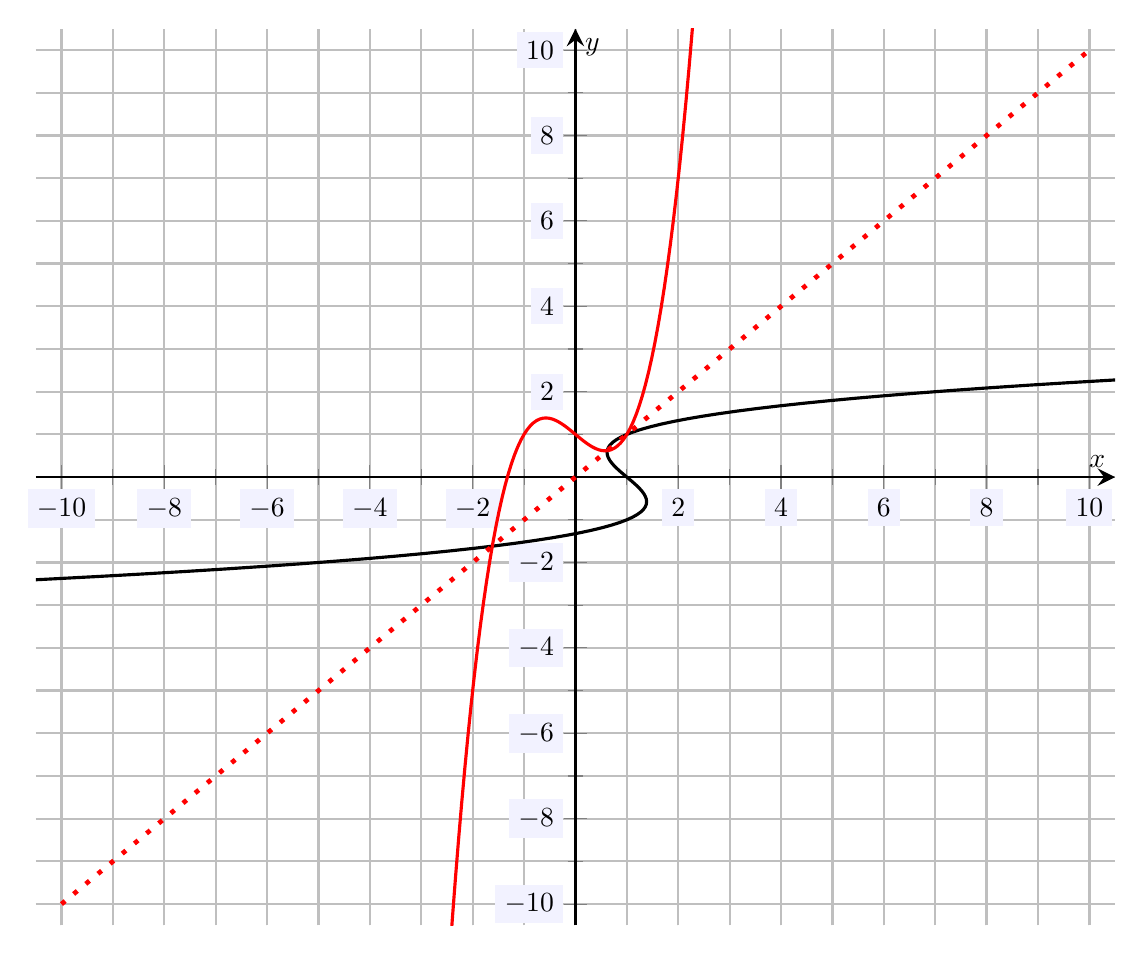
\begin{tikzpicture}[scale=2,every node/.style={scale=0.5}]
	\begin{axis}[
	grid=both,
	axis lines=middle,
	ticklabel style={fill=blue!5!white},
	xmin= -10.5, xmax=10.5,
	ymin= -10.5, ymax=10.5,
	xtick={-10,-8,-6,-4,-2,0,2,4,6,8,10},
	ytick={-10,-8,-6,-4,-2,0,2,4,6,8,10},
	minor tick = {-10,-9,...,10},
	xlabel=\(x\),ylabel=\(y\),
	]
	\addplot[line width= 0.02cm,domain= -3:3, samples=100] ({x^3 - x +1},{x});
	\draw[red, dotted, line width= 0.03cm] (-10,-10) -- (10,10);
	\addplot[red,line width= 0.02cm,domain= -3:3, samples=100] ({x}, {x^3 - x +1});
	\end{axis}
	\end{tikzpicture}
	}
	\] \pspace

{\noindent \itshape Because the relation above passes the horizontal line test, i.e. every horizontal line intersects the function at most once, the relation has an inverse function. To sketch the inverse, we reflect the curve through the line $y= x$ (the dotted red line shown above). This yields the solid red curve shown above.}



% Question 8
\newpage
\question[10] As accurately as possible, sketch the line $2x - 3y= 6$ on the plot below. Your plot should include at least three points that are exactly on the line. 
	\[
	\fbox{
	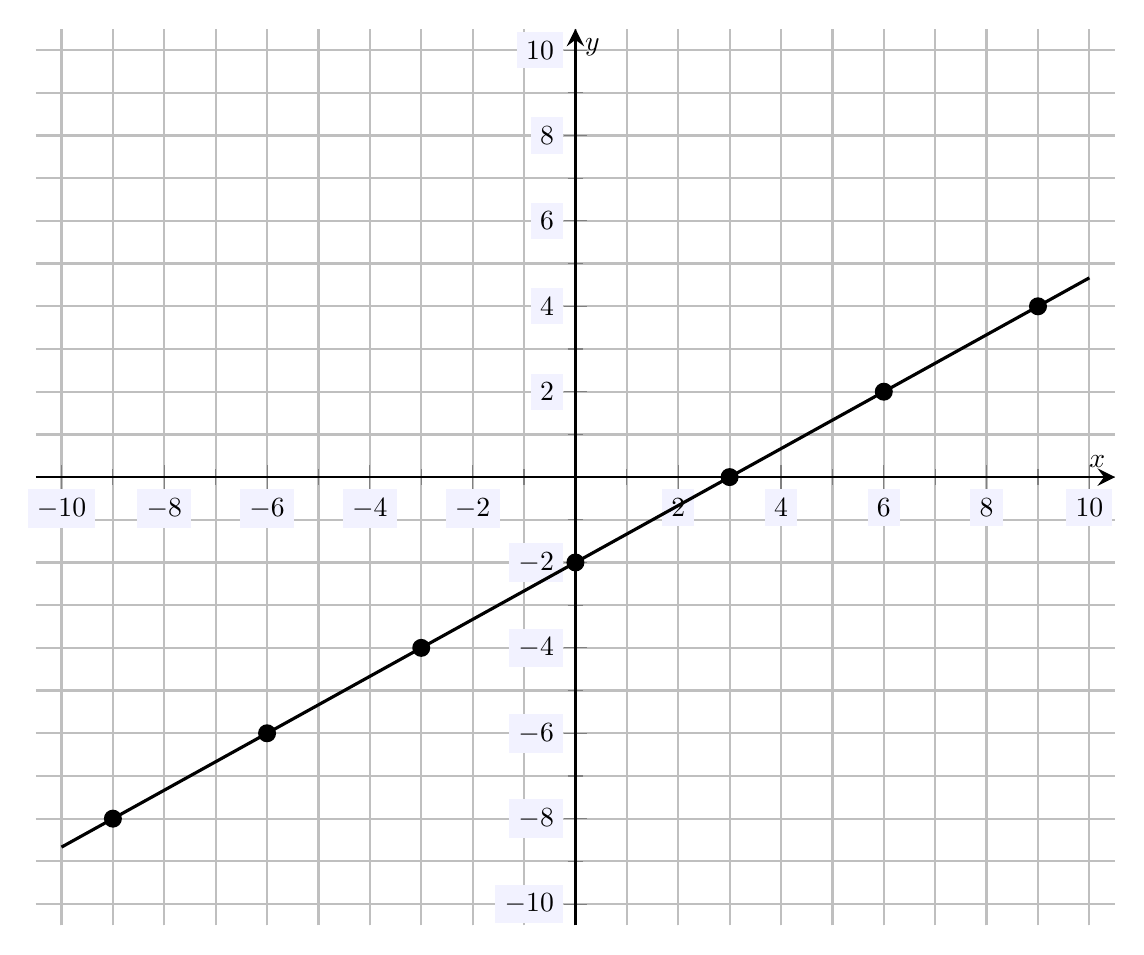
\begin{tikzpicture}[scale=2,every node/.style={scale=0.5}]
	\begin{axis}[
	grid=both,
	axis lines=middle,
	ticklabel style={fill=blue!5!white},
	xmin= -10.5, xmax=10.5,
	ymin= -10.5, ymax=10.5,
	xtick={-10,-8,-6,-4,-2,0,2,4,6,8,10},
	ytick={-10,-8,-6,-4,-2,0,2,4,6,8,10},
	minor tick = {-10,-9,...,10},
	xlabel=\(x\),ylabel=\(y\),
	]
	\addplot[line width= 0.02cm,domain= -10:10] ({x}, {2/3*x - 2});
	
	\draw[fill=black] (0, -2) circle (0.05cm);
	%
	\draw[fill=black] (3, 0) circle (0.05cm);
	\draw[fill=black] (6, 2) circle (0.05cm);
	\draw[fill=black] (9, 4) circle (0.05cm);
	%
	\draw[fill=black] (-3, -4) circle (0.05cm);
	\draw[fill=black] (-6, -6) circle (0.05cm);
	\draw[fill=black] (-9, -8) circle (0.05cm);
	
	\end{axis}
	\end{tikzpicture}
	}
	\] \pspace

{\noindent \itshape Solving for $y$ in $2x - 3y= 6$, we have\dots
	\[
	\begin{aligned}
	2x - 3y&= 6 \\[0.3cm]
	-3y&= -2x + 6 \\[0.3cm]
	y&= \dfrac{2}{3}\,x - 2
	\end{aligned}
	\]
Therefore, the line has slope $m= \dfrac{2}{3}$ and $y$-intercept, $(0, -2)$. Interpreting the slope $m= \dfrac{2}{3}$ as $\dfrac{\Delta y}{\Delta x}$, we see that for every increase of 3 in $x$ results in an increase of 2 in $y$. Alternatively, interpreting the slope $m= \dfrac{2}{3}= \dfrac{-2}{-3}$ as $\dfrac{\Delta y}{\Delta x}$, we see that for every decrease of 3 in $x$ results in a decrease of 2 in $y$. Using these interpretations beginning at the point $(0, -2)$, we can sketch the seven points shown in the plot above. Connecting this smoothly, we obtain the line $2x - 3y= 6$. 
}



% Question 9
\newpage
\question[10] Determine whether the table of values below could be given by a linear function. If not, explain why. If it can, find the linear function.
        \begin{table}[!ht]
        \centering
        \begin{tabular}{|c || r | r | r |} \hline
	$x$ & $0.2$ & $3.6$ & $5.1$ \\ \hline
	$y$ & $9.84$ & $-1.38$ & $-6.33$ \\ \hline
        \end{tabular}
        \end{table} \pspace

{\noindent \itshape A linear function has a constant rate of change, i.e. a constant slope. We can compute the slope by taking the points pairwise:
	\[
	\begin{aligned}
	m&= \dfrac{9.84 - (-1.38)}{0.2 - 3.6}= \dfrac{11.22}{-3.4}= -3.3 \\[0.3cm]
	m&= \dfrac{-1.38 - (-6.33)}{3.6 - 5.1}= \dfrac{4.95}{-1.5}= -3.3
	\end{aligned}
	\]
Because the slope is constant, the function given by the table above is linear. We know that the function has the form $y= mx + b$. The slope, $m$, is $-3.3$ so that $y= -3.3x + b$. The point $(0.2, 9.84)$ is on the graph of the function. Then when $x= 0.2$, we know that $y= 9.84$. We then have\dots
	\[
	\begin{aligned}
	y&= -3.3x + b \\[0.3cm]
	9.84&= -3.3(0.2) + b \\[0.3cm]
	9.84&= -0.66 + b \\[0.3cm]
	b&= 10.5
	\end{aligned}
	\]
Therefore, the linear function is $y= -3.3x + 10.5$. 
	\[
	\boxed{y= -3.3x + 10.5}
	\]
}



% Question 10
\newpage
\question[10] Determine whether the following lines are the parallel, perpendicular, or neither. Be sure to justify your answer. 
	\[
	\begin{aligned}
	\ell_1 &\colon & 2x - y&= 5 \\[0.3cm]
	\ell_2 &\colon & -2x + 4y&= 24
	\end{aligned}
	\] \pspace

{\noindent \itshape Solving for $y$ in each linear equation, we have\dots
	\[
	\begin{aligned}
	2x &- y= 5 & \qquad -2x &+ 4y= 24 \\[0.3cm]
	-y&= -2x + 5 & 4y&= 2x + 24 \\[0.3cm]
	y&= 2x - 5 & y&= \dfrac{1}{2}\,x + 6
	\end{aligned}
	\]
The slope of the first line is $m_1= 2$ and the slope of the second line is $m_2= \frac{1}{2}$. Because $m_1 \neq m_2$, the lines cannot be parallel. Therefore, the lines intersect. However, the negative reciprocal of $m_1$ is $-\frac{1}{2} \neq m_2$. Therefore, the lines are not perpendicular. Therefore, the lines are neither parallel nor perpendicular. 
}



% Question 11
\newpage
\question[10] Consider the line $4x - 6y= 12$.
	\begin{enumerate}[(a)]
	\item Determine the slope of the given line.
	\item Interpret the slope in at least two different ways.
	\item Is the function whose graph is the given line an increasing or decreasing function? Explain. 
	\item Determine the $y$-intercept of the given line. 
	\item Determine the $x$-intercept of the given line. 
	\end{enumerate} 

{\itshape
\sol
\begin{enumerate}[(a)]
\item Solving for $y$ in $4x - 6y= 12$, we have\dots
	\[
	\begin{aligned}
	4x &- 6y= 12 \\
	-6y&= -4x + 12 \\
	y&= \dfrac{2}{3}\,x - 2
	\end{aligned}
	\]
Because the line is in the form $y= mx + b$, we have $m= \frac{2}{3}$ and $b= -2$. Therefore, the slope is $m= \frac{2}{3}$. 

\item From (a), we know that $m= \frac{2}{3}$. Thinking of the slope as $\frac{\Delta y}{\Delta x}$, we can see that every increase of 3 in $x$ results in an increase of 2 in $y$. Equivalently, using the fact that $m= \frac{2}{3}= \frac{-2}{-3}$, we can see that every decrease of 3 in $x$ results in a decrease of 2 in $y$. Alternatively, using the fact that $m= \frac{2}{3} \approx 0.6667= \frac{0.6667}{1}$, we can see that every increase of 1 in $x$ results in an increase of 0.6667 in $y$. Alternatively, using the fact that $m \approx 0.6667= \frac{0.6667}{1}= \frac{-0.6667}{-1}$, we can see that every decrease of 1 in $x$ results in a decrease of 0.6667 in $y$. 

\item From (a), we know that the slope is $m= \frac{2}{3} > 0$. Because $m > 0$, $y$ is an increasing function of $x$. 

\item The $y$-intercept of a function occurs when $x= 0$. But then\dots
	\[
	\begin{aligned}
	4x - 6y&= 12 \\
	4(0) - 6y&= 12 \\
	-6y&= 12 \\
	y&= -2
	\end{aligned}
	\]
Therefore, the $y$-intercept is $-2$, i.e. $(0, -2)$. 

\item The $x$-intercept of a function occurs when $y= 0$. But then\dots
	\[
	\begin{aligned}
	4x - 6y&= 12 \\
	4x - 6(0)&= 12 \\
	4x&= 12 \\
	x&= 3
	\end{aligned}
	\] 
Therefore, the $x$-intercept is $3$, i.e. $(3, 0)$. 
\end{enumerate}
}



% Question 12
\newpage
\question[10] A caterer charges a flat fee for each person for whom a meal has to be prepared. The caterer charges \$270 for 15 people and \$360 for 20 people. Let $C(p)$ denote the cost of hiring the caterer to prepare food for $p$ people. 
	\begin{enumerate}[(a)]
	\item Explain why $C(p)$ is linear.
	\item Find $C(p)$.
	\item Interpret the slope of $C(p)$ in the context of the problem. 
	\item Find and interpret $C(32)$. 
	\end{enumerate} \pspace

{\itshape
\begin{enumerate}[(a)]
\item Because the caterer charges a flat fee per person, i.e. constant fee, the rate of change of the total amount charged by the caterer, $C(p)$, is constant. Therefore, $C(p)$ is a linear function. \pspace

\item We know that the caterer charges \$270 for 15~people, i.e. the graph of $C(p)$ contains the point $(15, 270)$, and \$360 for 20~people, i.e. the graph of $C(p)$ contains the point $(20, 360)$. Because $C(p)$ is linear, we know that $C(p)= mp + b$. Now\dots
	\[
	m= \dfrac{\Delta C}{\Delta p}= \dfrac{360 - 270}{20 - 15}= \dfrac{90}{5}= 45
	\]
But then $C(p)= 45p + b$. Because $(15, 270)$ is on the line, we know that $C= 270$ when $p= 15$. Then we have\dots
	\[
	\begin{aligned}
	C(p)&= 45p + b \\[0.3cm]
	270&= 45(15) + b \\[0.3cm]
	270&= 675 + b \\[0.3cm]
	b&= -405
	\end{aligned}
	\]
Therefore, $C(p)= 45p - 405$. \pspace

\item Because $C(p)= 45p - 405$ is of the form $y= mx + b$, the slope of $C(p)$ is $m= 45$. Thinking of this as $m= \frac{\Delta C}{\Delta p}$, we see that for every increase of one person, the caterer charges \$45 more; that is, the caterer charges \$45 per person. \pspace

\item We have\dots
	\[
	C(32)= 45(32) - 405= 1440 - 405= 1035
	\]
This implies that the caterer charges \$1,035 for preparing meals for 32~people. 
\end{enumerate}

\vfill Note. One would expect that the caterer charges \$0 for 0~people. But the points $(0, 0)$, $(15, 270)$, and $(20, 360)$ do not all lie along a line. An argument can be made that $C(p)$ cannot be linear. However, one could also assume that the caterer has a minimum number of people required so that $C(p) > 0$---in this case 10~people ($C(9)= 0$). Then the caterer charges \$45 for each additional person beyond the ninth person. 
}



% Question 13
\newpage
\question[10] A certain species of fungus reproduces by releasing tiny spores. The larger the fungus, the more spores that are released. Scientist find that the number of spores (in thousands) a fungus with diameter $d$ (in inches) can be modeled by $N(d)= -3.5 + 15.5d$.
	\begin{enumerate}[(a)]
	\item Find and interpret the slope of $N(d)$ in the context of the problem.
	\item Find and interpret in the context of the problem, if possible, the $y$-intercept of $N(d)$.
	\item According to the model, how large would the fungus have to be in order for it to release 100,000 spores?
	\end{enumerate} \pspace

{\itshape
\sol
\begin{enumerate}[(a)]
\item We know that the slope of $N(d)= -3.5 + 15.5d$ is $m= 15.5$. Interpreting this as $\dfrac{\Delta N}{\Delta d}$, we see that every increase of 1~in in diameter results in an increase by 15.5~thousand spores released; that is, the fungus releases 15,500~spores more for every inch wider that it is. \pspace

\item The $y$-intercept of $N(d)= -3.5 + 15.5d$ is $-3.5$, i.e. $(0, -3.5)$. This would imply that a fungus with a diameter of 0~in releases $-3.5$~spores. But it makes no sense for a fungus to have a diameter of 0~in, i.e. no size at all. In addition, it does not make sense for the fungus to release negative spores. Therefore, there is no interpretation in context. \pspace

\item If the fungus releases 100,000~spores, i.e. 100~thousand, then $N(d)= 100$. But then we have\dots
	\[
	\begin{aligned}
	N(d)&= 100 \\[0.3cm]
	-3.5 + 15.5d&= 100 \\[0.3cm]
	15.5d&= 103.5 \\[0.3cm]
	d&= 6.68
	\end{aligned}
	\]
Therefore, the fungus would have to have a diameter of 6.68~in. 
\end{enumerate}
}



% Question 14
\newpage
\question[10] Showing all your work, find the equation of the line whose $x$-intercept is $(-1, 0)$ that has slope $-\frac{6}{7}$. \pspace

{\noindent \itshape Because the desired line is not vertical, it must have the form $y= mx + b$. We know that the slope is $-\frac{6}{7}$, i.e. $m= -\frac{6}{7}$. We then know that $y= -\frac{6}{7}\,x + b$. We know that the $x$-intercept of the line is $(-1, 0)$, i.e. the line contains the point $(-1, 0)$. But then when $x= -1$, we know that $y= 0$. Then we have\dots
	\[
	\begin{aligned}
	y&= -\dfrac{6}{7}\,x + b \\[0.3cm]
	0&= -\dfrac{6}{7} \cdot -1 + b \\[0.3cm]
	0&= \dfrac{6}{7} + b \\[0.3cm]
	b&= -\dfrac{6}{7}
	\end{aligned}
	\]
Therefore, the line is $y= -\frac{6}{7}\,x - \frac{6}{7}= -\frac{6}{7} (x + 1)$. 
	\[
	\boxed{y= -\dfrac{6}{7}\,x - \dfrac{6}{7}}
	\]
}



% Question 15
\newpage
\question[10] Showing all your work, find the equation of the line that is parallel to the line $x= 4$ that contains the $y$-intercept of the line $-6x + 5y= 11$. \pspace

{\noindent \itshape Because the desired line is parallel to the line $x= 4$, which is a vertical line, the desired line must also be a vertical line. Therefore, the desired line has the form $x= c$ for some $c$. But we know that the desired line contains the $y$-intercept of the line $-6x + 5y= 11$. However, the $y$-intercept occurs when $x= 0$. But then the line must be the line $x= 0$.
	\[
	\boxed{x= 0}
	\]
}



% Question 16
\newpage
\question[10] Showing all your work, find the equation of the line that is perpendicular to the line $y= 6 - 7x$ at its $y$-intercept. \pspace

{\noindent \itshape We know that the desired line is not perpendicular. Therefore, the desired line has the form $y= mx + b$. Because the desired line is perpendicular to this line, its slope is the negative reciprocal of the slope of $y= 6 - 7x$, which is $-7= -\frac{7}{1}$. Therefore, $m= \frac{1}{7}$ so that $y= \frac{1}{7}x + b$. We know also the desired line contains the $y$-intercept of $y= 6 - 7x$. The $y$-intercept of $y= 6 - 7x$ is $(0, 6)$. Therefore, the desired line contains the point $(0, 6)$, i.e. when $x= 0$, $y= 6$. But then\dots
	\[
	\begin{aligned}
	y&= \dfrac{1}{7}\,x + b \\[0.3cm]
	6&= \dfrac{1}{7} \cdot 0 + b \\[0.3cm]
	b&= 6
	\end{aligned}
	\]
Therefore, the line is $y= \frac{1}{7}\,x + 6$. \pspace
	\[
	\boxed{y= \dfrac{1}{7}\;x + 6}
	\]
}



% Question 17
\newpage
\question[10] Showing all your work, solve the following equation and then verify your solution:
	\[
	6 \left( \dfrac{1}{2}\,x + 5 \right)= 28
	\] \pvspace{1.5cm}

{\itshape
	\[
	\begin{aligned}
	6 \left( \dfrac{1}{2}\,x + 5 \right)&= 28 \\[0.3cm]
	3x + 30&= 28 \\[0.3cm]
	3x&= -2 \\[0.3cm]
	x&= -\dfrac{2}{3}
	\end{aligned}
	\] \pspace
We can verify the solution: \pspace
	\[
	\begin{aligned}
	6 \left( \dfrac{1}{2}\,x + 5 \right)&= 28 \\[0.3cm]
	6 \left(\dfrac{1}{2} \cdot -\dfrac{2}{3} + 5 \right) &\stackrel{?}{=} 28 \\[0.3cm]
	6 \left(-\dfrac{1}{3} + 5 \right) &\stackrel{?}{=} 28 \\[0.3cm]
	6 \left(-\dfrac{1}{3} + \dfrac{15}{3} \right) &\stackrel{?}{=} 28 \\[0.3cm]
	6 \cdot \dfrac{14}{3} &\stackrel{?}{=} 28 \\[0.3cm]
	2 \cdot \dfrac{14}{1} &\stackrel{?}{=} 28 \\[0.3cm]
	28&= 28 \\
	&\text{ \cmark}
	\end{aligned}
	\]
}



% Question 18
\newpage
\question[10] Showing all your work, solve the following equation:
	\[
	7x + 4= 6 - 2(3 - x)
	\] \pvspace{1.5cm}

	\[
	\begin{aligned}
	7x + 4&= 6 - 2(3 - x) \\[0.3cm]
	7x + 4&= 6 - 6 + 2x \\[0.3cm]
	7x + 4&= 2x \\[0.3cm]
	4&= -5x \\[0.3cm]
	x&= -\dfrac{4}{5}
	\end{aligned}
	\]



% Question 19
\newpage
\question[10] Showing all your work, solve the following equation:
	\[
	\sqrt{2} \left( x - \sqrt{2} \right)= \dfrac{x + 5}{3}
	\] \pvspace{1.5cm}

	\[
	\begin{aligned}
	\sqrt{2} \left( x - \sqrt{2} \right)= \dfrac{x + 5}{3} \\[0.3cm]
	\sqrt{2}\,x - 2= \dfrac{x + 5}{3} \\[0.3cm]
	3(\sqrt{2}\,x - 2)= \dfrac{x + 5}{3} \cdot 3 \\[0.3cm]
	3\sqrt{2}\,x - 6= x + 5 \\[0.3cm]
	3\sqrt{2}\,x - x - 6= 5 \\[0.3cm]
	3\sqrt{2}\,x - x= 11 \\[0.3cm]
	(3\sqrt{2} - 1)x= 11 \\[0.3cm]
	x= \dfrac{11}{3\sqrt{2} - 1}
	\end{aligned}
	\]



% Question 20
\newpage
\question[10] Showing all your work, solve the following equation:
	\[
	\dfrac{x + 6}{1 - x}= 10
	\] \pvspace{1.5cm}

	\[
	\begin{aligned}
	\dfrac{x + 6}{1 - x}&= 10 \\[0.3cm]
	x + 6&= 10(1 - x) \\[0.3cm]
	x + 6&= 10 - 10x \\[0.3cm]
	11x + 6&= 10 \\[0.3cm]
	11x&= 4 \\[0.3cm]
	x&= \dfrac{4}{11}
	\end{aligned}
	\]


\end{questions}
\end{document}